
\chapter{数据复制和共识协议}

数据复制和共识模块是构建高可用和容错能力强大的分布式系统的基石。
在Apache IoTDB中,数据复制和共识协议由共识模块实现。
本节将会介绍IoTDB的共识模块,阐述IoTDB的统一共识模块的设计考量,详细介绍三个不同一致性级别的共识算法实现:RatisConsensus,IoTConsensus和IoTConsensusV2,并且给出每一个共识算法的可用性保障语义。


\section{共识模块概述}

在Apache IoTDB中,共识模块是构建高可用能力和故障容错能力的基石。IoTDB的所有核心功能,无论是用户数据的管理,还是集群元数据的维护,乃至负责全局服务配置和协调的ConfigNode服务,都依赖共识模块提供的能力。

共识模块的核心目标在于为同一份数据维护多个满足一致性要求的数据副本。这种数据副本的能力是是抵御单点故障、实现自动容错能力的直接基础,也是负载均衡、节点扩缩容等高级功能的前提。
从自动容错的角度来看,当某个存储数据的节点发生宕机或网络不可达时,系统可以依赖其他副本上的数据继续对外提供服务,从而避免了数据丢失和服务中断。
从负载均衡和扩缩容的角度来看,应用可以选择将读请求分散到不同的副本上,有效提升系统的并发处理能力;在需要进行节点维护或集群规模调整时,共识协议负责在节点之间实现副本数据的搬运,保证数据不丢失的前提下安全地迁移数据和调整节点数量。

在对内的实现上,共识模块隐藏了数据副本同步和一致性维护过程中所面临的诸多复杂挑战,包括但不限于高效地进行数据的同步/异步复制,如何保障每一个副本在故障情况下都能在最终状态上保持高度一致,如何在网络波动下的实现数据的断点续传,如何处理并发写入时可能出现的数据冲突并根据预设的解决策略确保一致性等内容。

对外而言,共识模块的抽象极大地简化了上层依赖模块的开发工作。
对于数据写入模块而言,它不需要关心底层数据是如何同步到多个副本的,只需要向任何一个副本的共识模块提交写入请求即可,共识模块保证了请求返回时数据已经达到一致性级别的复制。这种简化降低了写入模块的复杂性,使其可以更专注于业务逻辑的实现。
对于数据查询模块来说,查询引擎可以放心地从任意一个可用的副本读取数据,并能够确保读取到的数据满足系统所定义的一致性级别。
这种设计上的解耦不仅降低了开发难度,也提升了系统的整体可维护性和可扩展性。


\section{共识模块统一框架}

IoTDB内部的不同应用模块需要依赖不同级别的共识协议,这种需求驱动了IoTDB建立统一的共识模块框架,通过可配置可插拔的共识协议来满足不同应用模块的需求,并为系统未来集成新的共识协议提供了扩展性。

\begin{figure}
    \centering
    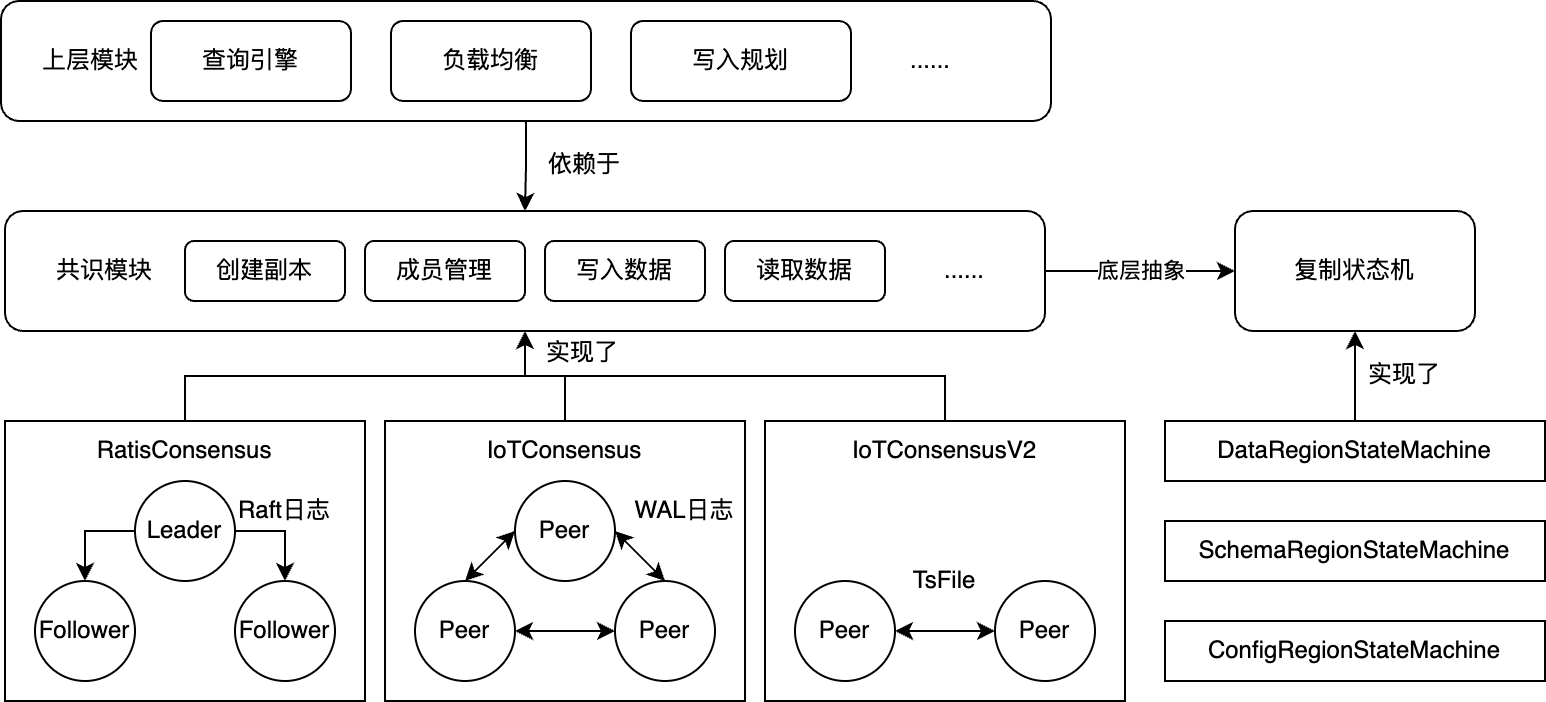
\includegraphics[width=0.99\linewidth]{c04-consensus-arch.png}
    \caption{共识层统一框架架构图}
    \label{fig:c04-consensus-arch}
  \end{figure}
  
图\ref{fig:c04-consensus-arch} 给出了共识模块统一框架的示意图。

共识模块要求所有的上层服务遵循复制状态机(replicated state machine)\cite{lamport1978statemachine}的规范。目前,实现了复制状态机规范的包括了存储引擎DataRegionStateMachie,元数据存储引擎SchemaRegionStateMachine和集群分区和管理服务ConfigRegionStateMachine。

共识模块定义了针对数据副本组的标准接口,包括创建和销毁数据副本、在数据副本上执行写入操作、从数据副本中读取数据、对数据副本的数量、组成成员进行变更等能力。

目前IoTDB中实现了共识模块标准接口的共识协议有三种,分别是基于Raft算法的强一致性共识协议RatisConsensus,基于多主复制的会话一致性共识协议IoTConsensus和基于主从快照同步的最终一致性共识协议IoTConsensusV2。

本章节的剩下部分会介绍每一种共识协议的实现细节。


\section{RatisConsensus}

RatisConsensus是IoTDB提供的强一致性共识协议实现,基于Raft共识算法和Apache Ratis\cite{ratis}开源项目实现。由于RatisConsensus给出了强一致性的语义保障,目前已成为集群元数据管理和ConfigNode分区服务默认的共识协议。

RatisConsenus内部会维护奇数(2n+1,默认为3)个副本,并为每一个副本提供强一致性的语义保障。由于底层依赖的Raft算法是基于单主复制结构的共识协议,因此在任何时刻,这些副本只有一个可以接受上层的写入请求,被称为Leader副本,剩下节点从Leader副本同步数据,可以接受只读请求。
RatisConsensus能够自动容忍少数副本的失效依然保持数据和服务的可用性。具体来说,对于一个2n+1副本的RatisConsensus服务,最多能够容忍n个副本的失效。同时,RatisConsensus能够保证在网络分区情况下的数据一致性,同一时刻能保证最多只有一个副本成为Leader副本。
当Leader副本失效之后,RatisConsensus内部存在自动故障转移的机制,通过新一轮的内部选举在短时间内(默认4-8秒)选出一个新的Leader副本。

RatisConsensus底层的一致性协议是Raft算法,包含Leader选举、日志复制和安全性保障等核心要素。Raft通过随机超时来实现Leader选举,通过任期(Term)来保证每次选举的唯一性和权威性。Leader接受写入数据,并将自身日志强制复制给所有Follower,最终所有的日志可以被排列出一个副本之间达成共识的全序序列,不同的副本均按照这个全序序列应用日志,从而实现副本数据之间的一致性。为了确保安全性,Raft 引入了 Commit 机制,即只有在大多数副本上保存了对应日志条目后,该日志才能被 Commit,上层才能收到共识层写入成功的回应。

\begin{figure}
  \centering
  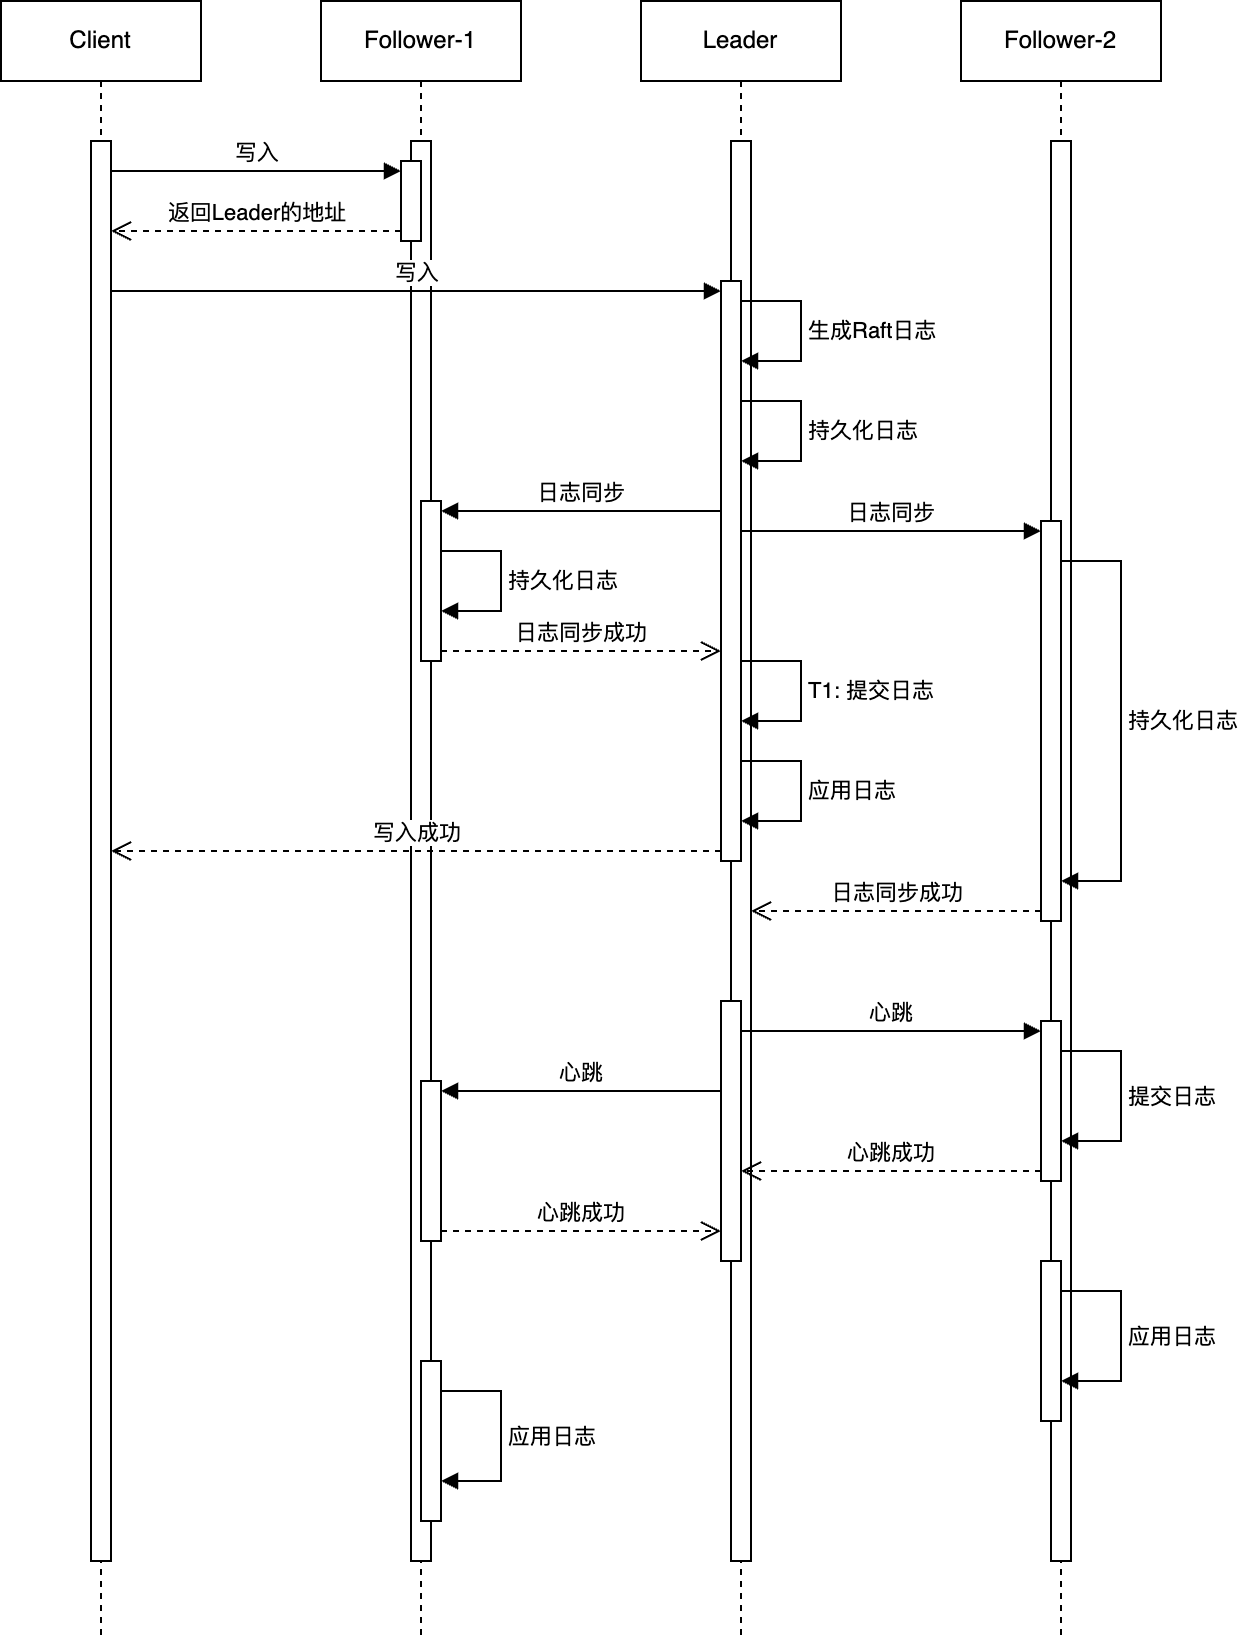
\includegraphics[width=0.7\linewidth]{c04-ratis-write.drawio.png}
  \caption{RatisConsensus数据写入和副本复制流程}
  \label{fig:c04-ratis-write}
\end{figure}

图\ref{fig:c04-ratis-write}给出了一条数据提交给RatisConsensus之后背后的数据复制流程。用户写入数据之后,会由Leader这边负责生成持久化日志并同步到所有节点上,在T1时刻,有超过半数的节点完成持久化同步之后,该操作的状态将会改变成Commit,Leader会应用这个日志并返回对应的结果。Raft算法会在后台保证所有节点能够最终都Commit并应用这个日志。



\section{IoTConsensus}

IoTConsensus是IoTDB提供的会话一致性共识协议实现,基于多主异步复制的自研实现,针对工业物联网时序场景写入模式有针对性的优化。目前,IoTConsensus是集群数据管理的可选共识协议之一。

IoTConsensus的设计初衷是为牺牲一定的可用性换取极致的可用性和更高的性能。
用于在工业物联网场景中,设备不断的时序数据,每台设备的写入请求往
往是串行无重复的,因而并发的写入请求之间通常不存在冲突。因此,IoTConsensus放宽了串形化的一致性约束,允许任何一个副本都能接受读写请求,并且请求在一个副本上执行成功即可返回客户端操作成功。


\begin{figure}
  \centering
  \subcaptionbox{IoTConsensu整体结构\label{fig:c04-iot-arch}}
    {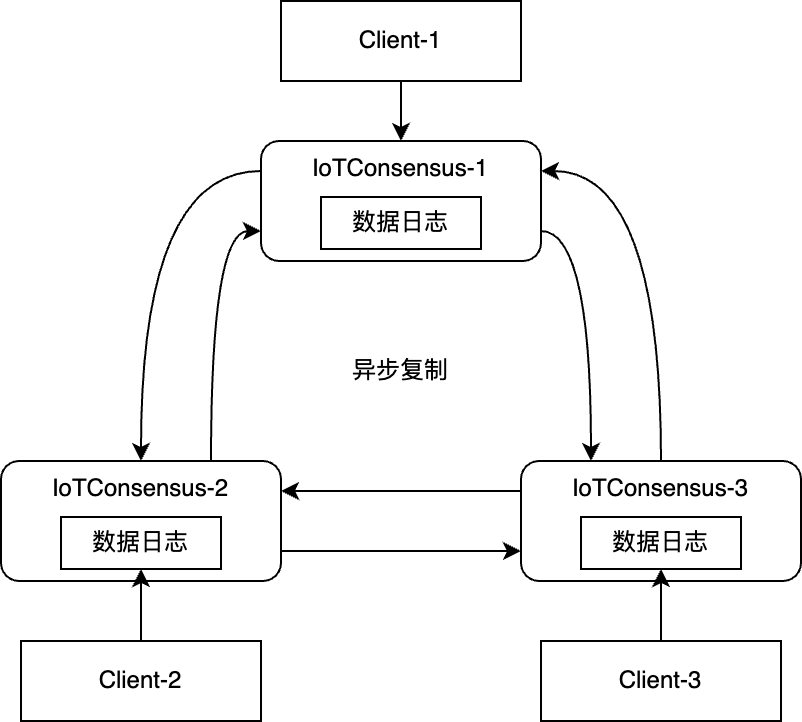
\includegraphics[width=0.4\linewidth]{c04-iot-arch.png}}
  \subcaptionbox{IoTConsensus写入流程\label{fig:c04-iot-write}}
    {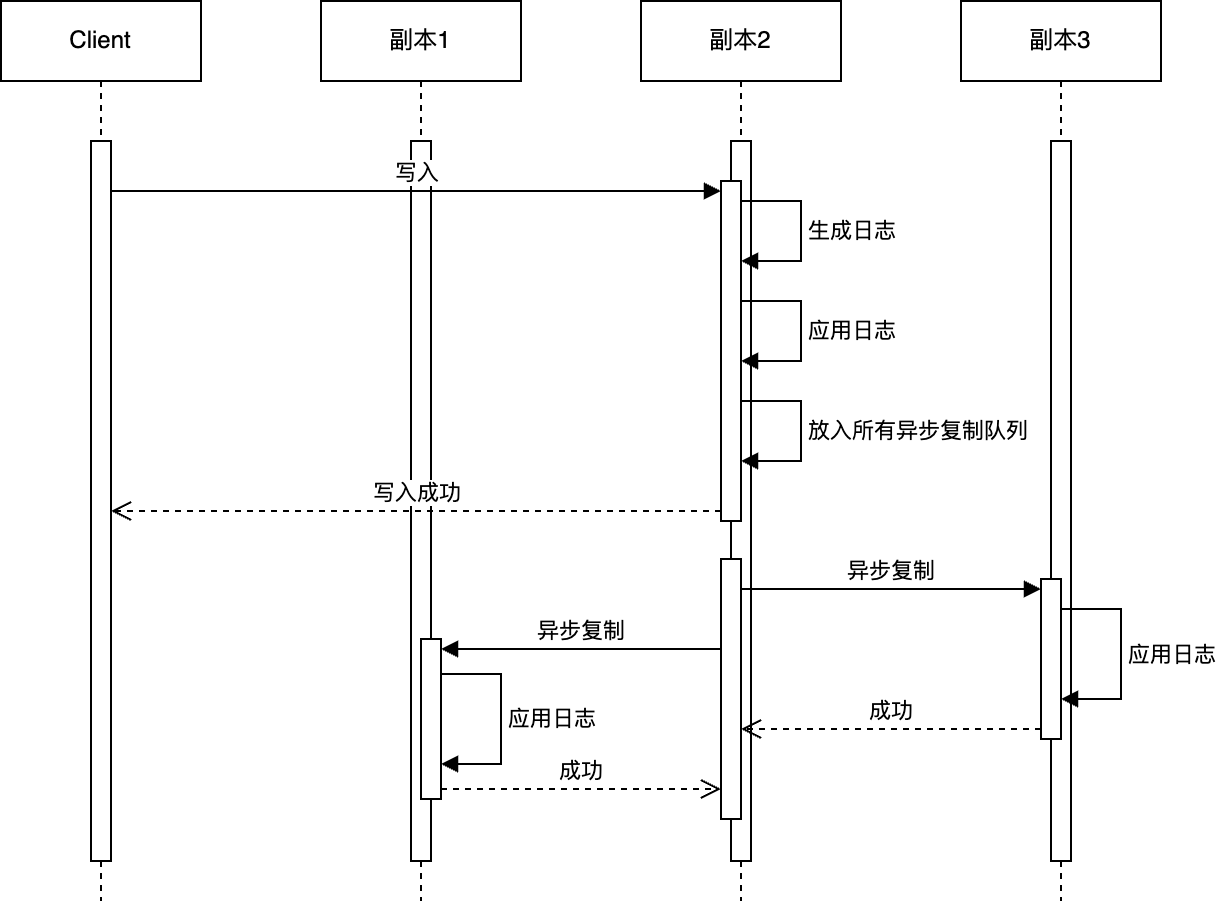
\includegraphics[width=0.58\linewidth]{c04-iot-write.png}}
  \caption{IoTConsensus示意图}
  \label{fig:c04-iot-consensus}
\end{figure}

图\ref{fig:c04-iot-arch}展示了IoTConsensus的结构,允许任何一个副本接受客户端的写入请求,并通过每个节点的后台异步复制线程将写入请求通过WAL的方式同步给其他的副本。


值得注意的是,当不同副本的数据产生冲突是,可能会导致副本之间数据无法达到最终一致,该问题的解决需要应用层的介入。例如在 Apache IoTDB 中,如果观察到某个序列的数据在不同副本上不一致,则可以使用 Select Into 子句拉取该序列在当前 Leader 副本上的数据并
重新向该共识组流式写入。但在绝大部分的正常应用场景,这种不一致不会发生。

虽然IoTConsensus支持多个副本的同时并发写入,但在实践过程中,为了提高性能、降低并发冲突,ConfigNode会为IoTConsensus挑选一个名义意义上的“主副本”,并默认将所有的写入请求引导到这个请求上。当“主副本”发生故障时,ConfigNode会启动故障容错和恢复机制,推举一个新的副本成为名义“主副本”。


\section{IoTConsensusV2}

IoTConsensusV2是IoTDB提供的最终一致性共识协议实现,基于主从异步复制的自研实现,针对工业物联网时序场景写入模式有针对性的优化。目前,IoTConsensusV2是集群数据管理的可选共识协议之一。

IoTConsensusV2相较于IoTConsensus相比,进一步牺牲了副本之间的同步时延、一致性级别,换取了极高的写入吞吐。IoTConsensusV2的总体思路是允许在部分场景下使用TsFile进行副本间的数据同步。基于TsFile的同步过程仅涉及到常数级别的复杂度操作,同时不用经过 WAL 的磁盘持久化和 Memtable 的内存维护,因此写入吞吐非常高,并且能够解决IoTConsensus存在的由于Follower宕机或Leader节点写入速率大于同步速率导致的WAL文件堆积和写入阻塞的问题。

然而,TsFile的生成相比每一条写入日志需要较长的时间,副本间数据同步延迟在极端环境下可达到几十分钟甚至是几个小时的数据。在两副本的情况下,如果主副本宕机,可能出现由于部分数据还未同步导致的数据暂时丢失的情况。如果宕机节点后续永久没有加入集群,那么这部分数据就会永久丢失。

\begin{figure}
    \centering
    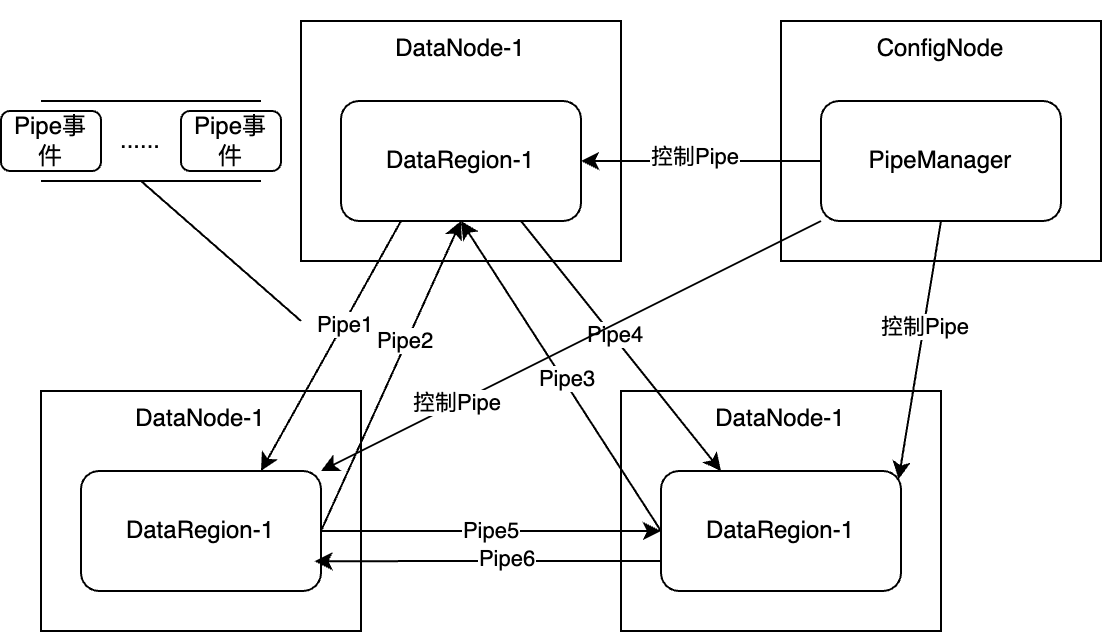
\includegraphics[width=0.8\linewidth]{c04-pipe-consensus.png}
    \caption{IoTConsensusV2的整体结构}
    \label{fig:c04-pipe-consensus}
  \end{figure}
  
图\ref{fig:c04-pipe-consensus}给出了IoTConsensusV2的整体架构。IoTConsensusV2具备以下两种同步模式:

1. Stream传输模式。在默认状态下使用WAL进行数据同步,来达到更快的同步速度和更高的一致性。当WAL堆积或者TsFile堆积的场景下,切换到TsFile进行数据传输,来达到更低的资源消耗和更高的吞吐。

2. Batch传输模式。该模式下,所有的数据同步都通过TsFile实现。

和IoTConsensus相似,ConfigNode也会为IoTConsensusV2挑选一个名义意义上的“主副本”,并默认将所有的写入请求引导到这个请求上。当“主副本”发生故障时,ConfigNode会启动故障容错和恢复机制,推举一个新的副本成为名义“主副本”。


\section{共识模块总结}

下表给出了共识模块三个共识协议的对比。

\begin{table}
    \centering
    \caption{共识协议对比}
    \begin{tabular}{cccc}
      \toprule
      特性         & RatisConsensus & IoTConsensus &  IoTConsensusV2 \\
      \midrule
      副本一致性级别   & 线性一致性 & 会话一致性 &  最终一致性 \\
       副本复制策略    & 半同步    & 异步       & 异步       \\
       自动故障转移    &  内部选举    &   ConfigNode指定    &  ConfigNode指定  \\ 
      共识协议结构   & 主从 & 多主 &  多主  \\
      数据同步性能   & 一般 & 较高 &  极高  \\
      \bottomrule
    \end{tabular}
    \label{tab:consensus-compare}
  \end{table}



